\section{Introduction}
\label{introduction}

%\todo[inline]{stress the timing aspect more}
Implantable medical devices such as pacemakers are designed to improve physiological conditions with very little human intervention. 
Their ability to autonomously affect the physiological state of the patient makes the medical devices safety-critical, and sufficient evidence for their safety and efficacy should be provided before the devices can be implanted in the patients. Medical devices increasingly rely on software, and device function and their clinical performance can be affected by seemingly minor changes to software.
%As more functionality is added to the devices
\footnote{In what follows, the word `device' is used to refer to the software of the device.}
%, the complexity of the software component of the device is increasing dramatically, leading to a large number of potential safety violations because of software bugs. 

Over the course of the past four decades, cardiac rhythm management devices such as pacemakers and implantable cardioverter defibrillators (ICD) have grown in complexity and now have more than 80,000 to 100,000 lines of software code~\cite{pauljones}. In 1996, 10\% of all medical device recalls were caused by software-related issues and this rose to 15\% between 2003-2012~\cite{recall_stats,killedbycode}. There is currently no standard for testing, validating, and verifying the software for implantable medical devices.

There are two categories of device bugs: 
1) the device may fail to conform to its \emph{specifications}, that is, the prescription of how it should react to certain inputs.  
2) the device may fail to improve the conditions of the patient as promised, even if it conforms to its specifications. 
The desired physiological conditions that the closed-loop system should achieve are captured in the \emph{physiological requirements}; for example, for a pacemaker, the heart rate should always be maintained above a certain threshold. 
%In what follows, the word `requirement' always refers to such physiological requirements.
%Note that requirements are about \emph{the closed-loop system}: they prescribe the behavior of both device and environment (e.g. both pacemaker and heart).

Bugs in the first category (non-conformance to specification) can be detected via systematic and extensive open-loop testing in which a set of input sequences is fed to the device, and its output is compared with the expected output.
Bugs in the second category (violation of physiological requirements), on the other hand, require the availability of the \emph{closed-loop system}, which consists of the device and its environment.
For instance, the pacemaker and the heart as its environment. 
In the medical device industry, closed-loop verification of the physiological requirements is mostly performed in terms of clinical trials, in which the actual devices are implanted in human subjects over an extended duration.
Unfortunately, because of the extremely high cost of clinical trials (\$0.30
million to \$24.03 million~\cite{trial_cost}. with cardiac devices closer to the higher end), the amount and variety of human subjects during the clinical trials are limited, which reduces the opportunity to find bugs. 
Moreover, clinical trials are often conducted at the final design stage. Fixing bugs at this stage is very costly.

Closed-loop model checking enables closed-loop evaluation of the physiological requirements at an earlier design stage, which requires formal model(s) of the physiological environment. 
%Depending on the formalism used to model the environment (and device) and the language used to express the requirements, this allows the usage of formal methods to perform the verification.
%Formal environment modeling introduces new challenges that do not arise when modeling the device alone, and this paper aims at addressing these issues in the context of pacemaker verification.
%In the rest of this paper, we speak therefore of pacemaker as the Device Under Verification (DUV) and of the heart as being the environment, but it is understood that the discussion carries more broadly, with possible domain-specific adjustments.
In closed-loop model checking, there is only one device model. 
However there can be a large number of environmental conditions which require different models to represent them. For instance, a heart with atrial flutter has an additional conduction pathway that is not available in a healthy heart, causing fast atrial rate. The timing and structural differences should be distinguished in corresponding heart models.
%\todo[inline]{should we give an example of a heart condition?}
A set of initial models of the environment can be constructed but the set is inherently incomplete because of the large number of environment conditions and their combinations. 
As a result, performing model checking using every model in the set cannot ensure full coverage of the environmental conditions. 

In this paper, domain-specific over-approximation rules are developed that produce abstract models that not only cover explicitly modeled environment conditions, but also cover timing behaviors and conditions not modeled in the set of initial models. 
The abstract models can be then used for closed-loop model checking of the device model. 
If the closed-loop system satisfies a requirement, the device under verification satisfies the requirement under environment conditions covered by the abstract models. 
However, if the requirement is not satisfied, the model checker returns a counter-example. 
In device modeling, the counter-example is considered \emph{spurious} if it can not be produced by the device.
However in environment modeling, even if the counter-example can not be produced by any of the initial environment models, it might still be a physiologically valid behavior.
Thus the validity of a counter-example cannot be determined by refining the environment model, but can untimately only be determined by domain experts. 

Counter-examples returned from abstract models can be difficult to interpret by domain experts.
One abstract counter-example could be produced by multiple physiologically valid conditions, which causes ambiguity.
Thus, a rigorous framework is necessary to balance the need to cover a wide range of environmental conditions and the need to provide counter-examples to the physicians within their physiological context.

Another challenge for closed-loop model checking of medical devices is the amount of domain expertise needed during: 1) physiological modeling, 2) model abstraction and refinement, and 3) checking the validity of counter-examples.
Thus the framework must also allow non-domain experts to perform verification (item 2 above),
and establish `hand-off' points where the results of verification can be handed back 
to the experts for interpretation.

\begin{figure}[!t]
		\centering
		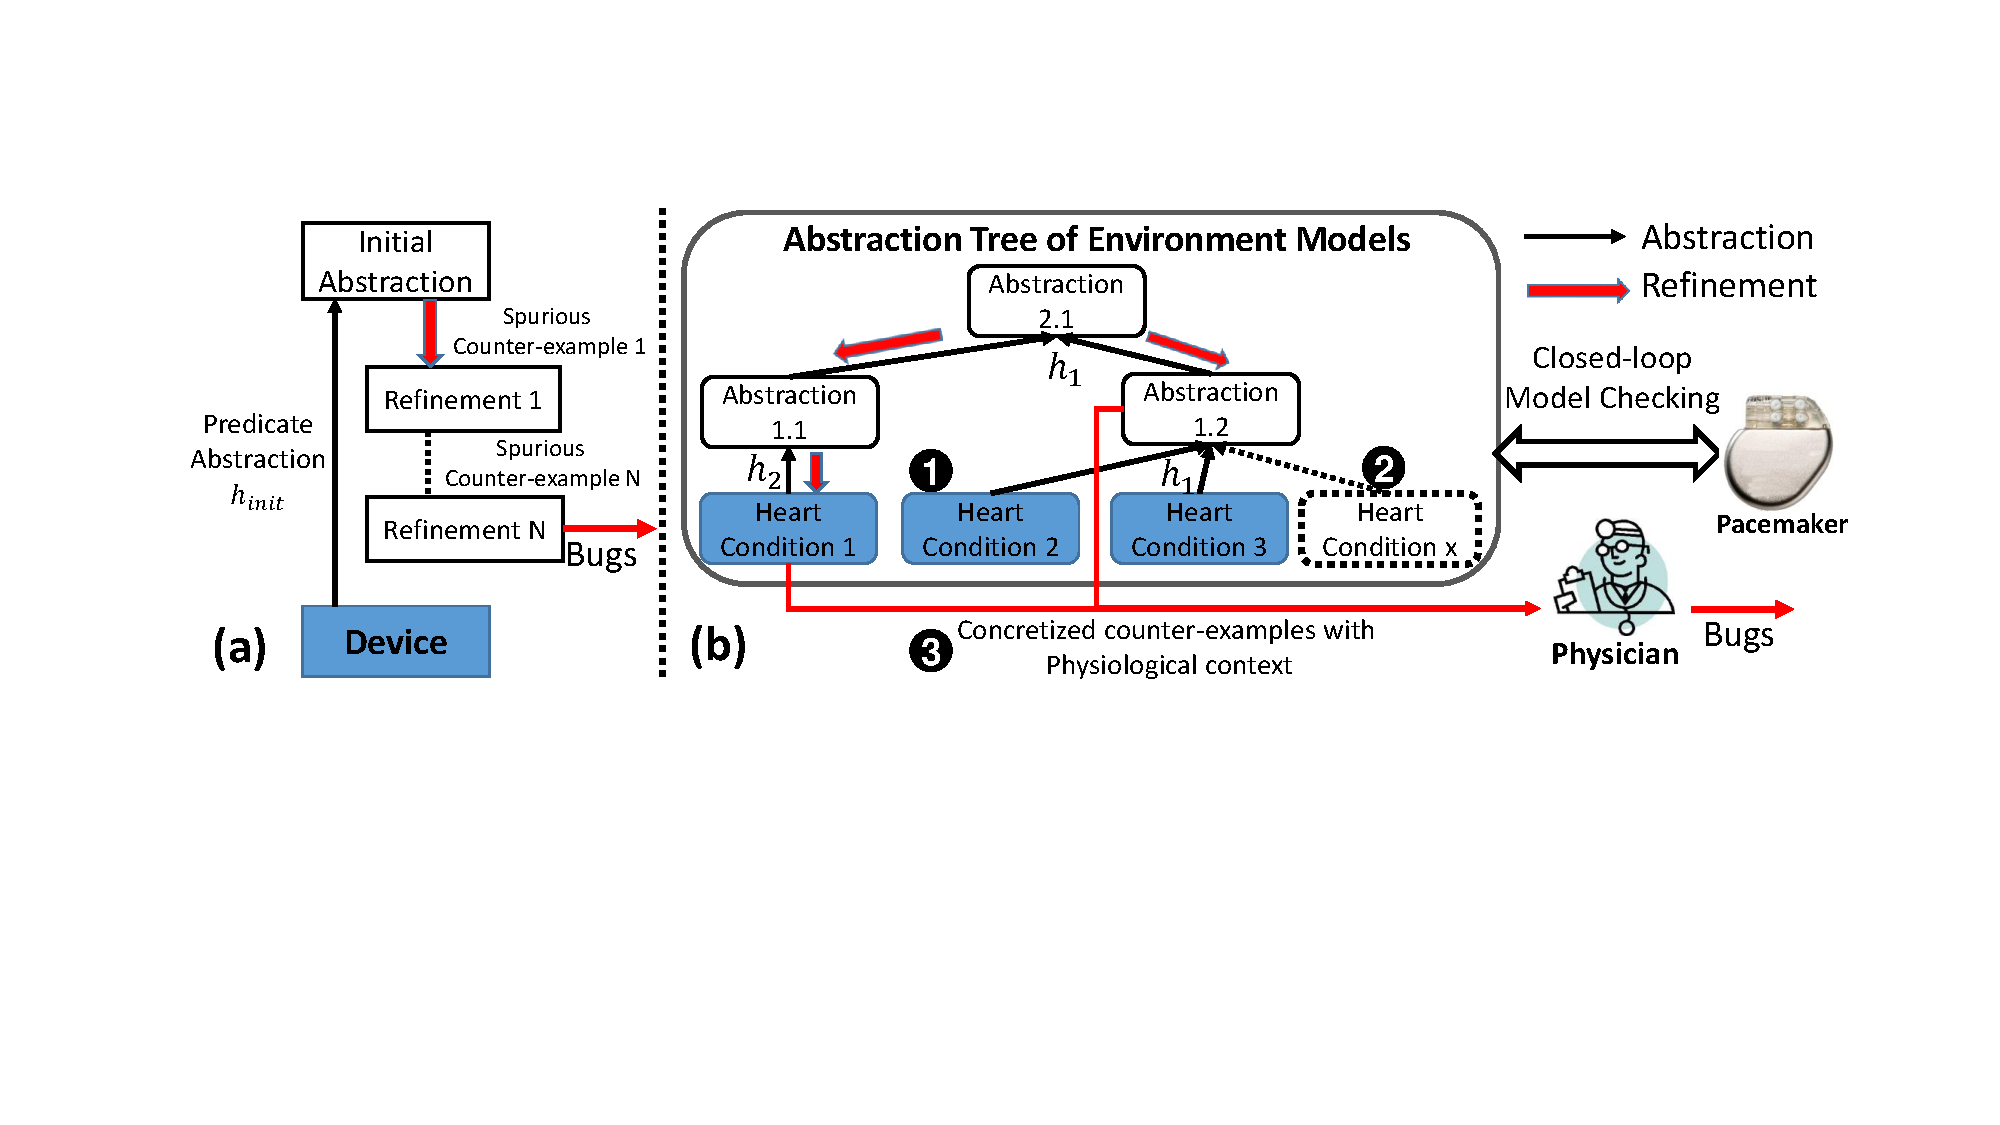
\includegraphics[width=\textwidth]{figs/distinction.pdf}
		%\vspace{-5pt}
		\caption{\small (a) Device modeling with CEGAR framework (b) Closed-loop model checking with environment abstraction tree.}% The initial set of heart conditions are first abstracted and/or merged using abstraction rules $h_1,h_2$ (Marker 1). The abstract model is first used for closed-loop model checking. When a property violation happens, refined models in the abstraction tree are used for model checking. The most concrete counter-examples may be available in the initial model(s) (Marker 2). In the scenario where counter-examples do not exist in explicitly modeled Heart condition 2 and 3, the counter-example in Abstraction 1.2 may correspond to a valid heart condition introduced during abstraction $h_1$. The physician decides the validity of the counter-examples.}
		  \vspace{-10pt}
		\label{fig:distinction}
\end{figure}


\subsection{Contributions}
In this paper a framework is proposed for environment modeling in closed-loop model checking of medical device software.
The cardiac pacemaker is used as an example of applying this framework.
An expandable set of timed-automata heart models are first developed to represent different physiological conditions (\figref{distinction} Marker 1).
A set of domain-specific abstraction rules are then developed based on physiological knowledge, which help ensure the physiological relevance of the behaviors introduced into the abstract models (\figref{distinction} Marker 2).
Then the rules are applied to the initial set of physiological models to obtain an abstraction tree, which will be used for closed-loop model checking of the pacemaker. 
A straightforward search procedure is then used to conduct model checking using suitable heart models and return the most concrete and unambiguous counter-examples to the physicians for analysis (\figref{distinction} Marker 3).
In this framework, physiological knowledge is only needed when constructing the initial model set and when analyzing counter-examples. 
The application of the physiological abstraction rules and the verification procedure can be automated.
The proposed method can potentially be generalized to other domains in which the device operates in a large variety of environmental conditions.
\subsection{Related Work}
%\todo[inline]{complete}
Counter-Example Guided Abstraction Refinement (CEGAR) \cite{CEGAR} has been proposed to over-approximate the device using predicate abstraction. (\figref{distinction}.(a))
%Upon property violation the abstract counter-example is checked for its validity on the actual system. If the counter-example is \emph{spurious} the model is then refined to eliminate the spurious counter-example. 
%This process is then continued on the refined model until either a valid counter-example returns or no counter-examples are returned. 
CEGAR works well during device modeling, however, it cannot be applied to environment modeling for two reasons: 1) predicate abstraction does not guarantee the validity of behaviors introduced into the model. In fact, for device modeling, all additional behaviors introduced into the abstract model are spurious. 2) the validity of a counter-example cannot be checked automatically as in device modeling. 

Physiological modeling of cardiac activities has been studied at different level for different applications. In \cite{natalia} the electrical activities of the heart are modeled in high spatial fidelity to study the mechanisms of cardiac arrhythmia. In \cite{radu} formal abstractions of cardiac tissue have been studied to reduce the complexity of the heart tissue model. However, these two models do not focus on the interaction with the pacemaker which cannot be used for closed-loop model checking. In \cite{marta} hybrid automata model of the heart has been used to capture the complex beat-to-beat dynamics of the heart tissue. However the model cannot be used to cover behaviors of multiple heart conditions.

In our previous work \cite{sttt13} a set of formal heart models covering various heart conditions at different abstraction levels were developed, and closed-loop model checking has been performed on models of implantable pacemakers. 
However the physiological knowledge required during each step of closed-loop model checking prevents the method to be practical.


%During the closed-loop model checking, the most abstract model(s) that are appropriate to the requirement are automatically selected as the initial environment models. If the requirement is satisfied, the system is safe under the environment conditions covered by the initial environment models. If the requirement is violated in certain initial environment model, the children of the model in the abstraction tree are used for model checking until 1) the leaves of the tree is reached, or 2) there is no violations in the child nodes. The counter-examples obtained at the most refined models are returned to the physician for validity check. This process is automated so that no domain knowledge is required for the person who performs model checking. It also ensures the most concrete counter-examples with unambiguous physiological context are returned to the physician for analysis. 
%The first challenge in closed-loop model checking of pacemakers is that the human heart displays a large number of different conditions, henceforth referred to as `physiological conditions'.
%E.g., one heart may display \emph{atrial fibrillation} where the upper chambers of the heart (the atria) produce an exceedingly fast beat that prevents proper blood pumping.
%Another heart may display Premature Ventricular Contraction (PVC) where a location in the ventricles produces electrical impulses at erratic time instants.\Hao{I don't think these two conditions make sense to the reader}
%Each such condition will require its own formal model, and some models may display more than one condition.
%In this paper, we build such a set of formal heart models using the timed automata formalism in Section ???.
%Performing model checking with each model separately, we seek a method that can combine models, and perform model checking on the merged model. 
%The combination of models must be such that if the merged model is correct (according to the requirements) then so is every model that was combined into it.
%We present \emph{abstraction rules} in Section ?? which allow us to do precisely that.

%This initial set of models will necessarily be \emph{incomplete} because the number of physiological conditions is too large, and some of the conditions are too ill-understood for modeling.
%Thus, unlike system modeling in which one typically starts from one ground truth model to be verified, our starting point is an \emph{incomplete set of environment models}.
%Because of this incompleteness, we seek abstraction rules that introduce new \emph{physiologically meaningful} behavior which might actually be produced by heart models not in the initial set.
%These then correspond to heart conditions not taken explicitly into account. 
%This provides a second motivation for the domain-specific abstraction rules $R$ in Section ???, which can be thought of as relaxations of the conditions governing the model's behavior. 
%Like predicate abstraction, they produce models that over-approximate the behavior of the model they are applied to (i.e., $\beh(R(M)) \supset \beh(M)$).
%However, the new behavior they introduce might not be spurious. 
%We demonstrate such a case in Section ???.
%If model checking returns a counter-example on $R(M)$, the physician can decide whether this is actually physiologically plausible behavior and therefore the pacemaker needs to be debugged, or this is indeed spurious and should be thrown out (and the abstraction refined).
%
%Note this is different from classical predicate abstraction [???], which adds behavior in a domain-agnostic fashion. In fact, predicate abstraction is a fist step in the timed automata model checking procedure as presented in [ALur and Dill 1994].
%Our abstraction rules are used to combine and and abstract models \emph{prior} to model checking.
%%tttt
%
%\subsubsection{Contributions}
%In this paper we propose a framework for environment modeling and model checking of medical device software, in particular, pacemakers.
%Specifically, we present several extended timed automata models of various heart conditions in Section ???. 
%We define domain-specific abstraction rules for these models, and demonstrate how these can be applied to gradually add physiologically meaningful behavior in Section ???. 
%Using the models and the rules, we build an abstraction tree which serves to perform model checking of physiological requirements for the heart+pacemaker closed loop in Section ???.
%We illustrate the approach via case studies in Section ???, and conclude in Section ???
%

%
